\documentclass[a4paper,11pt]{article}

\usepackage[utf8]{inputenc}
\usepackage[T1]{fontenc}
\usepackage[czech]{babel}
\usepackage{indentfirst}
\usepackage{graphicx}
\usepackage{tikz}
\usepackage{verbatim}

\title{Neužitečné informace k~projektu maticové kalkulačky}
\author{Přemysl Janouch}

\begin{document}
\maketitle

\begin{abstract}
Tento dokument slouží převážně k~účelu získání zápočtu z~předmětu TED, ale je velmi dobře možné, že se dozvíte i~něco o~mém semestrálním projektu na PA2. To bohužel zjistíte až na konci.
\end{abstract}

\section{Co to vlastně má být}
Vzhledem k~názvu \uv{maticová kalkulačka} lze oprávněně očekávat, že tento výtvor bude schopný provádět nějaké operace s~maticemi, jako je například násobení konstantou, sčítání a násobení matic stejného druhu, nebo takový výpočet determinantu. A abych to neměl tak jednoduché, dokonce mě donutili naimplementovat algoritmus pro Gaussovu eliminační metodu.

\subsection{Dobrovolná rozšíření}
Ačkoliv se po mně nechce nic příliš specifického a způsob provedení je do jisté míry volný k~rozvážení každého chudáka, který tento úkol dostal k~vypracování, rozhodl jsem se dosadit do programu pár mírně nadbytečných věcí, díky kterým bych z~něj měl mít o~trochu lepší pocit:

\begin{itemize}
\item řádkový vstup,
\item s~tím spojená \emph{infix} interpretace výrazů
\item a také operace sčítání a násobení dvou skalárů.
\end{itemize}

\section{A co to zase být nemá}
V~žádném případě neaspiruju na to, aby můj program dokázal vyhodnotit cokoliv třeba i~vzdáleně podobného následujícímu matematickému vzorečku:

\[e \cdot \frac{\lambda}{\sin \alpha} - 3 \cdot \det \textbf{A}^2 + \sqrt{3.1415926535897932384626}\]

Je přece jasné, že mám počítat matice a ne jakousi hloupou trigonometrii. Pozornému čtenáři taktéž neunikne, že s~číselnými operacemi v~použité přesnosti to také nebude na obyčejných počítačích zrovna jednoduché.

Zrovna tak se nedá očekávat podpora pro lineární operace z~vyšší dívčí, protože na takové ptákoviny\footnote{No pun intended.} nemám čas. Jeden příklad za všechny \cite{olsak}:

\[\frac{\left| \det \textbf{A} \right|}{\left\|(1, 0, -1)\times(3, 2, 1)\right\|}\]

\section{Návrh}
Tuto část textu jsem se rozhodl věnovat svému současnému plánu.

\subsection{Vzhled}
Představoval bych si, že program bude vypadat jako na obrázku \ref{fig:vzhled}. Je zřejmé, že půjde o~konzolovou aplikaci a snímek demonstruje zejména funkčnost.

\begin{figure}[h]
\centering
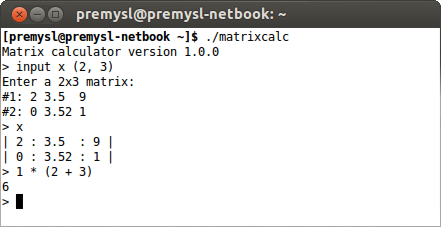
\includegraphics[width=0.6\textwidth]{screenshot.png}
\caption{Předpokládaný vzhled}
\label{fig:vzhled}
\end{figure}

\usetikzlibrary{arrows}

\subsection{Vnitřnosti}
Shodou okolností jsem se dostal až tak daleko, že vám rovněž mohu na tabulce \ref{tab:tridy} ukázat pár informací o~třídách, které se v programu vyskytnou:

\begin{table}[h]
\centering
\caption{Třídy v~programu}
\label{tab:tridy}
\begin{tabular}{ l l l }
\textbf{Název} & \textbf{Funkce} & \textbf{Bude těžká?} \\
\hline
Tokenizer & Scanner & Ani ne \\
Environment & Paměť pro proměnné atp. & Také ne \\
Value & Wrapper pro skalár nebo matici & Už vůbec ne \\
$\ast$EvalNode & Sada tříd vyhodnocovacího stromu & To samé \\
Matrix & Samotná matice & Hrozně!
\end{tabular}
\end{table}

\subsection{Gaussova eliminační metoda}
\emph{Gaussova eliminační metoda} je metoda usnadňující řešení soustav lin. rovnic. \cite{olsak} A to bude asi nejsložitější algoritmus v~celém programu. S~největší pravděpodobností použiju obdobný algoritmus, jako je v~\cite{wiki}:
\begin{verbatim}
for k = 1 ... m:
    # Find pivot for column k:
    i_max := argmax (i = k ... m, abs(A[i, k]))
    if A[i_max, k] = 0
        error "Matrix is singular!"
    swap rows(k, i_max)
    # Do for all rows below pivot:
    for i = k + 1 ... m:
        # Do for all remaining elements in current row:
        for j = k + 1 ... n:
            A[i, j] := A[i, j] - A[k, j] * (A[i, k] / A[k, k])
        # Fill lower triangular matrix with zeros:
        A[i, k] := 0
\end{verbatim}

\section{Závěrečné slovo}
Miluju \LaTeX{}! Do ničeho jiného nedokážete psát totální nesmysly tak, že to stejně vypadá krásně a seriózně. Můj vztah je plně vyjádřen obrázkem \ref{fig:tikz}.

\begin{figure}[h]
\centering
\begin{tikzpicture}[scale=0.5]
\fill[fill=red] (0,2) .. controls (0,0.5) and (2,1) .. (2,-0.5)
	.. controls (2,1) and (4,0.5) .. (4,2)
	.. controls (4,3.4) and (2,3.4) .. (2,2)
	.. controls (2,3.4) and (0,3.4) .. (0,2);
\draw (0,2) .. controls (0,0.5) and (2,1) .. (2,-0.5)
	.. controls (2,1) and (4,0.5) .. (4,2)
	.. controls (4,3.4) and (2,3.4) .. (2,2)
	.. controls (2,3.4) and (0,3.4) .. (0,2);
\end{tikzpicture}
\caption{Můj vztah k \LaTeX{}u}
\label{fig:tikz}
\end{figure}

\begin{thebibliography}{Olšák07}
\bibitem[Olšák07]{olsak}
	OLŠÁK, Petr:
	\emph{Úvod do algebry, zejména lineární.}
	Praha: FEL ČVUT, 2007. ISBN 978-80-01-03775-1.
\bibitem[Wiki]{wiki} Gaussian Elimination. In:
	\emph{Wikipedia: the free encyclopedia [online]}. St. Petersburg (Florida):
	Wikipedia Foundation, 16.~5.~2012, last modified on 10.~5.~2012.
	\par Dostupné z~\verb|http://en.wikipedia.org/wiki/Gaussian_elimination|
\end{thebibliography}

\end{document}


